% --- Generative simulators vs.\ JEPA ---
% % % --- Part E: JEPA / V-JEPA ---
% % \begin{frame}{JEPA: predict in embedding space, not pixels}
% %   \begin{itemize}\itemsep0.28em
% %     \item \textbf{Paradigm shift:} move from \textbf{generative reconstruction} (predict pixels) to \textbf{feature prediction}---learn latents by predicting \textbf{future or masked representations} while ignoring unpredictable nuisance variation (LeCun's JEPA blueprint).
% %     \item \textbf{I-JEPA / V-JEPA} (Meta): context encoder + predictor match \textbf{target-encoder} embeddings of masked spatio(-temporal) tokens; training signal lives in \textbf{representation space}.
% %     \item Connection to \textbf{world models}: both seek \textbf{abstract state} that supports forward prediction. Pure JEPA pretraining is often \textbf{representation SSL}; control stacks add \textbf{actions}, \textbf{rewards}, and \textbf{rollout-based RL} (Dreamer) or \textbf{action-conditioned} post-training (V-JEPA 2-AC, LeWM).
% %   \end{itemize}
% % \end{frame}

% % \begin{frame}{V-JEPA 2 / 2.1: scale, dense prediction, and robotics hooks}
% %   \begin{itemize}\itemsep0.28em
% %     \item[\textcolor{red}{$\blacktriangleright$}] \textbf{V-JEPA 2} scales masked latent video pretraining to internet-style data volumes and large encoders; \textbf{V-JEPA 2-AC} post-trains an \textbf{action-conditioned} head on small robot-trajectory corpora for \textbf{latent planning} and manipulation-style demos (see \href{https://arxiv.org/abs/2506.09985}{arXiv:2506.09985}).
% %     \item[\textcolor{red}{$\blacktriangleright$}] \textbf{V-JEPA 2.1} emphasizes \textbf{dense} self-supervision: masking objectives where \textbf{many tokens} (including visible context organization) shape the loss, plus deeper self-supervision across layers---aimed at finer spatial/temporal grounding (\href{https://arxiv.org/abs/2603.14482}{arXiv:2603.14482}).
% %     \item[\textcolor{red}{$\blacktriangleright$}] Conceptually: still \textbf{not} the same object as an RSSM with pixel decoder + RL losses, but increasingly aligned with \textbf{robotics world-model} pipelines that need \textbf{geometry and contact} in the latent.
% %   \end{itemize}
% %   \centering
% %   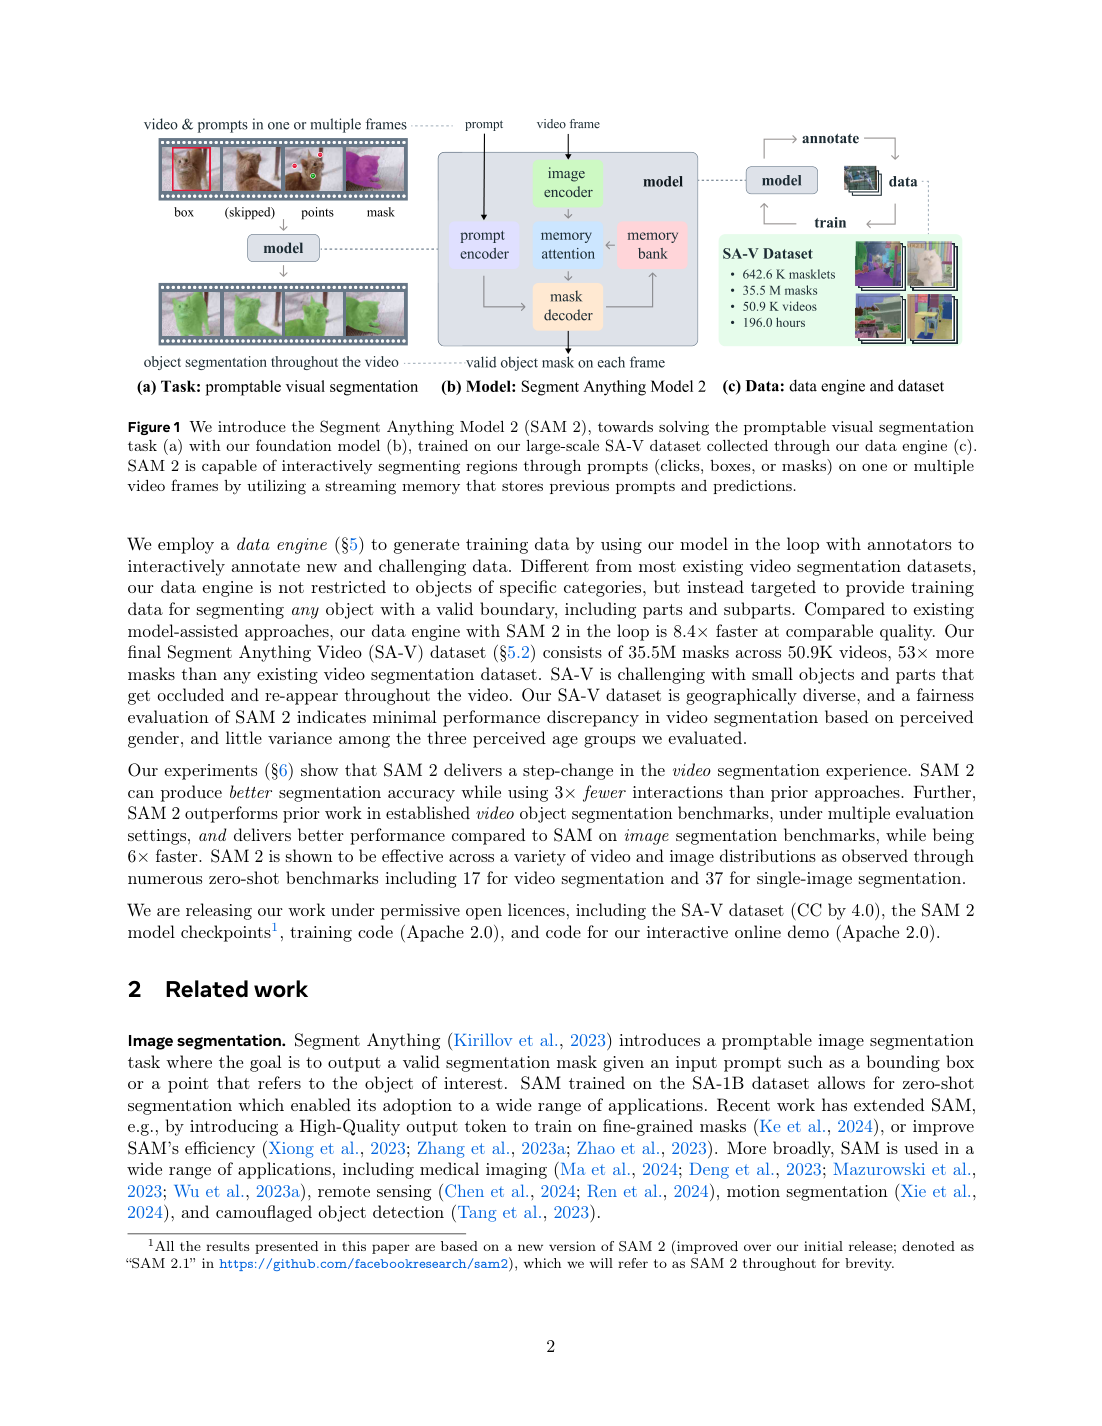
\includegraphics[width=\textwidth,height=0.40\textheight,keepaspectratio]{assets/New-Lecture_World_Models/vjepa_page_2.png}\\
% %   {\scriptsize Classic V-JEPA illustration; V-JEPA\,2/2.1 extend the same latent-prediction idea at scale.}
% % \end{frame}

% % \begin{frame}{Conceptual bridge: RSSM latents vs.\ JEPA embeddings}
% %   \begin{itemize}
% %     \item \textbf{RSSM} latents are trained for \textbf{reconstruction + RL} (reward, continuation); optimized to support \textbf{policy gradients through imagination}.
% %     \item \textbf{JEPA} targets are \textbf{invariance / prediction in feature space}; may align better with \textbf{semantics}, less with pixel-perfect physics unless combined with additional losses or fine-tuning.
% %     \item Active research: \textbf{action-conditioned JEPA}-style models for control (LeWM and successors push toward stable end-to-end training from pixels).
% %   \end{itemize}
% % \end{frame}
\begin{frame}[t]{Generative world models}
  \centering
  \includegraphics[width=0.76\linewidth,height=0.76\textheight,keepaspectratio]{assets/New-Lecture_World_Models/jepa_cs25_sl04_generative_world_models_sora_gaia.png}\\[0.04em]
  {\scriptsize Image credit: \href{https://drive.google.com/file/d/1bF5Yfzf-FG5iNIAgsXn2DwVD3l3ymvZW/view}{CS25}.}
\end{frame}

\begin{frame}[t]{Architectures: Generative v/s Joint Embedding}
  \centering
  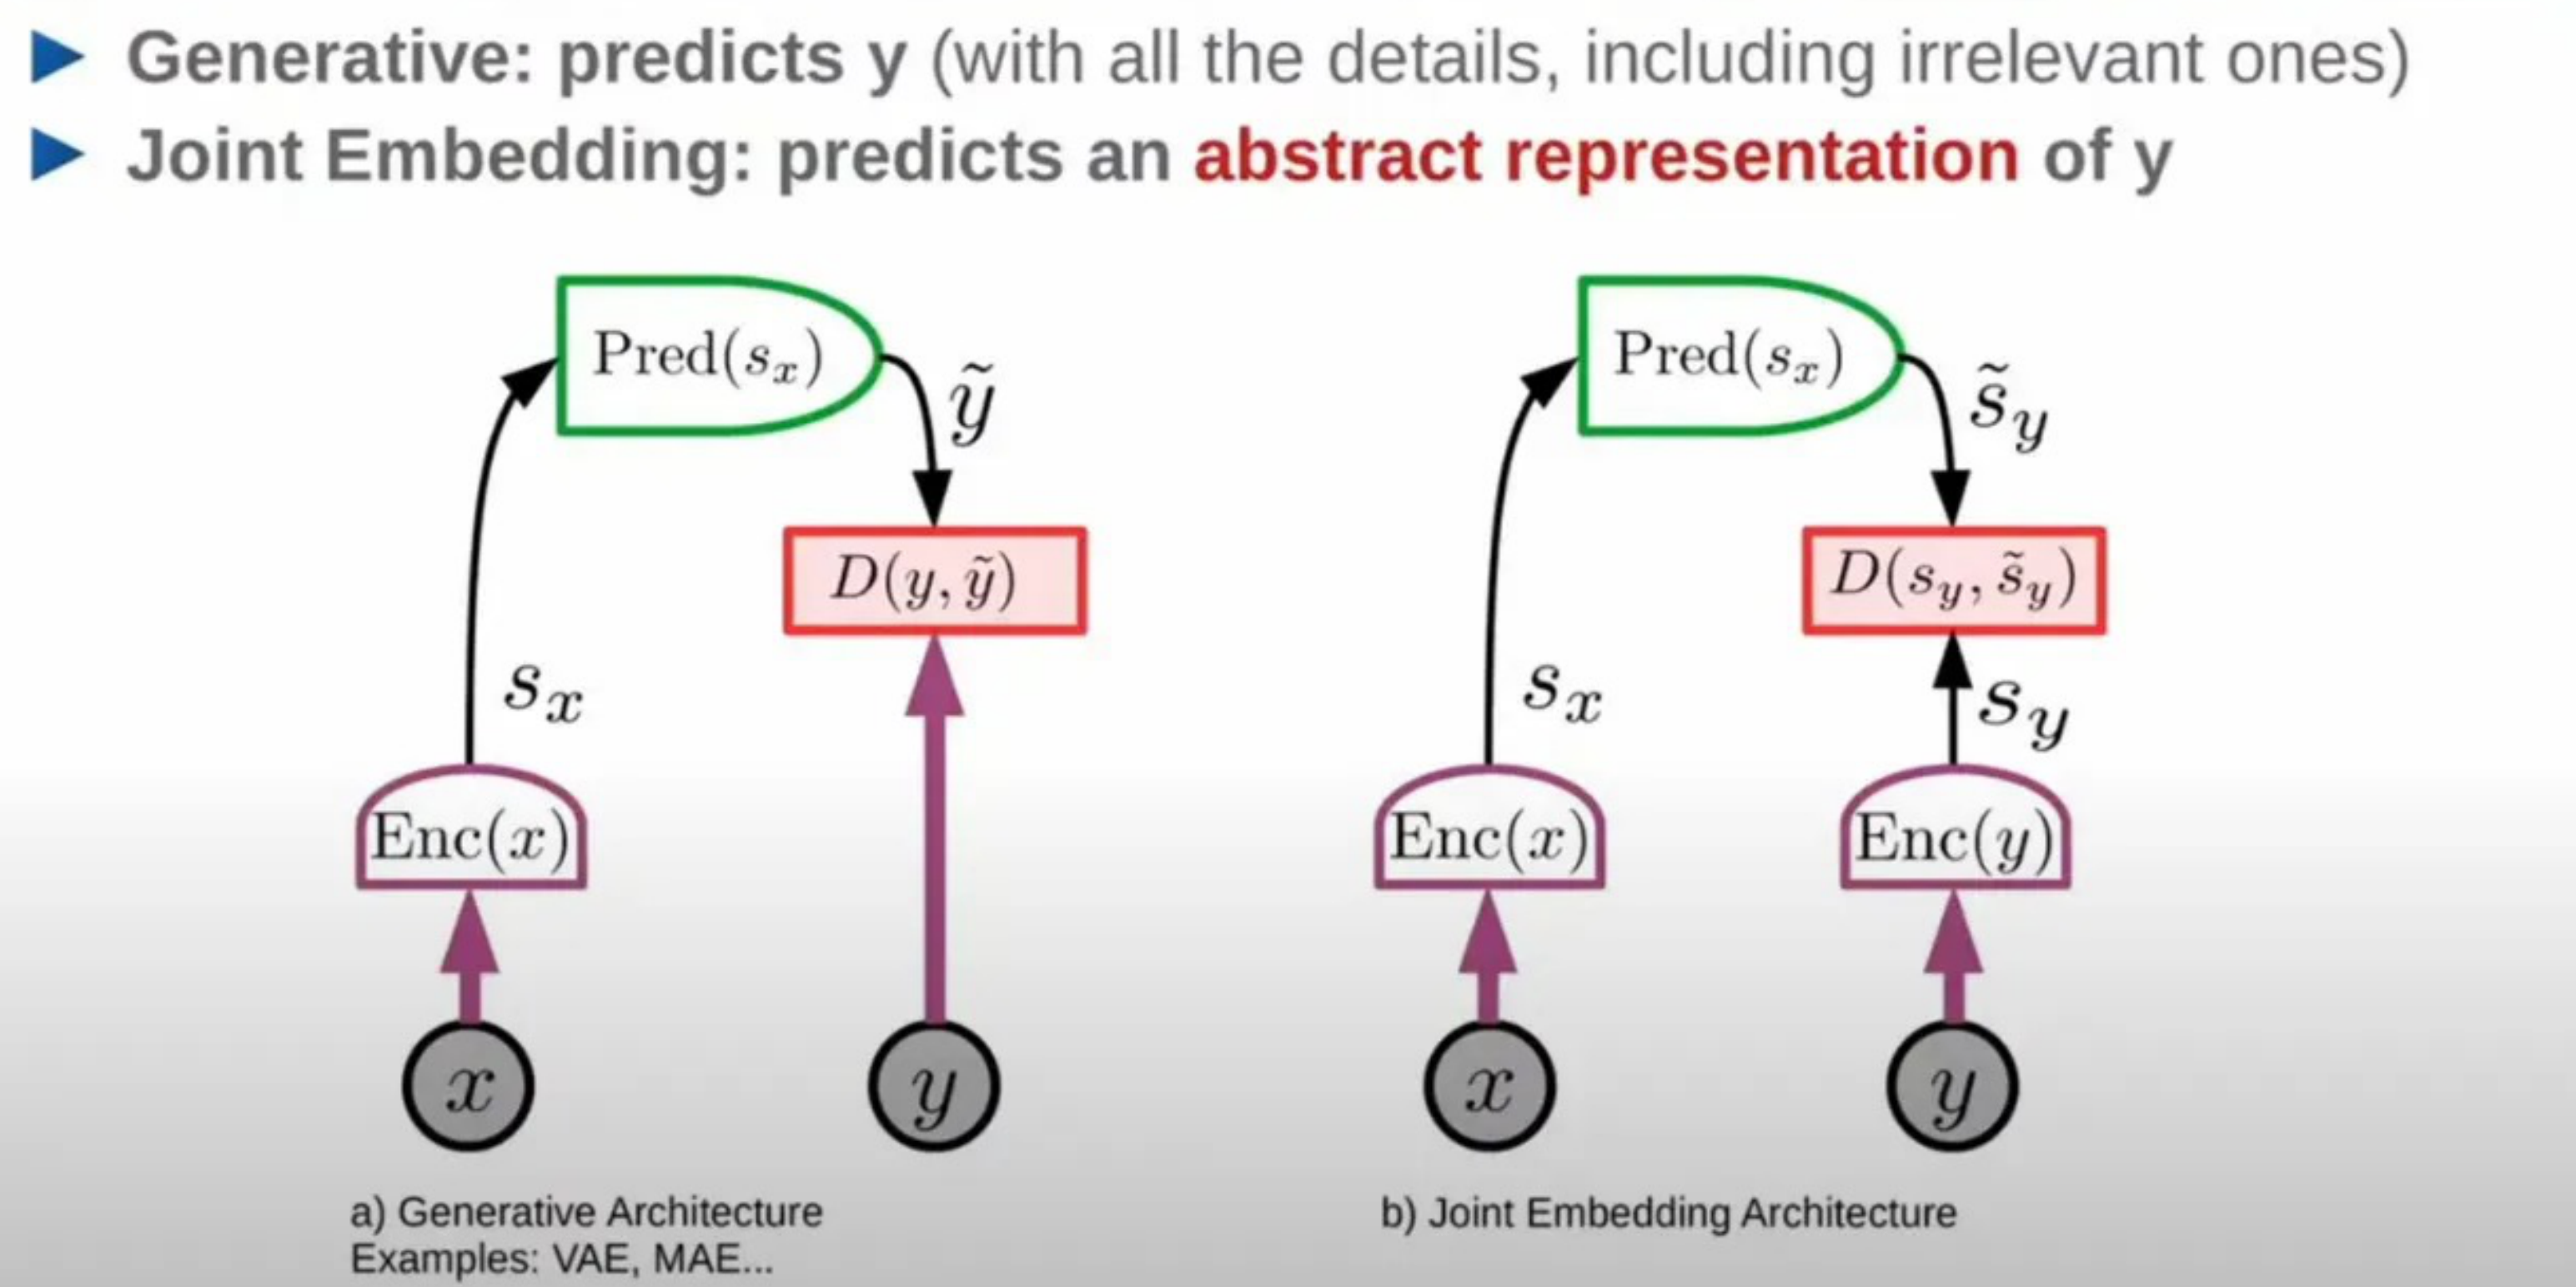
\includegraphics[width=\linewidth,height=0.82\textheight,keepaspectratio]{assets/New-Lecture_World_Models/jepa_cs25_sl05_lecun_world_model_figure.png}\\[0.08em]
  {\scriptsize Image credit: \href{https://drive.google.com/file/d/1bF5Yfzf-FG5iNIAgsXn2DwVD3l3ymvZW/view}{CS25}.}
\end{frame}

\begin{frame}[t]{JEPA \& energy-based view}
  \centering
  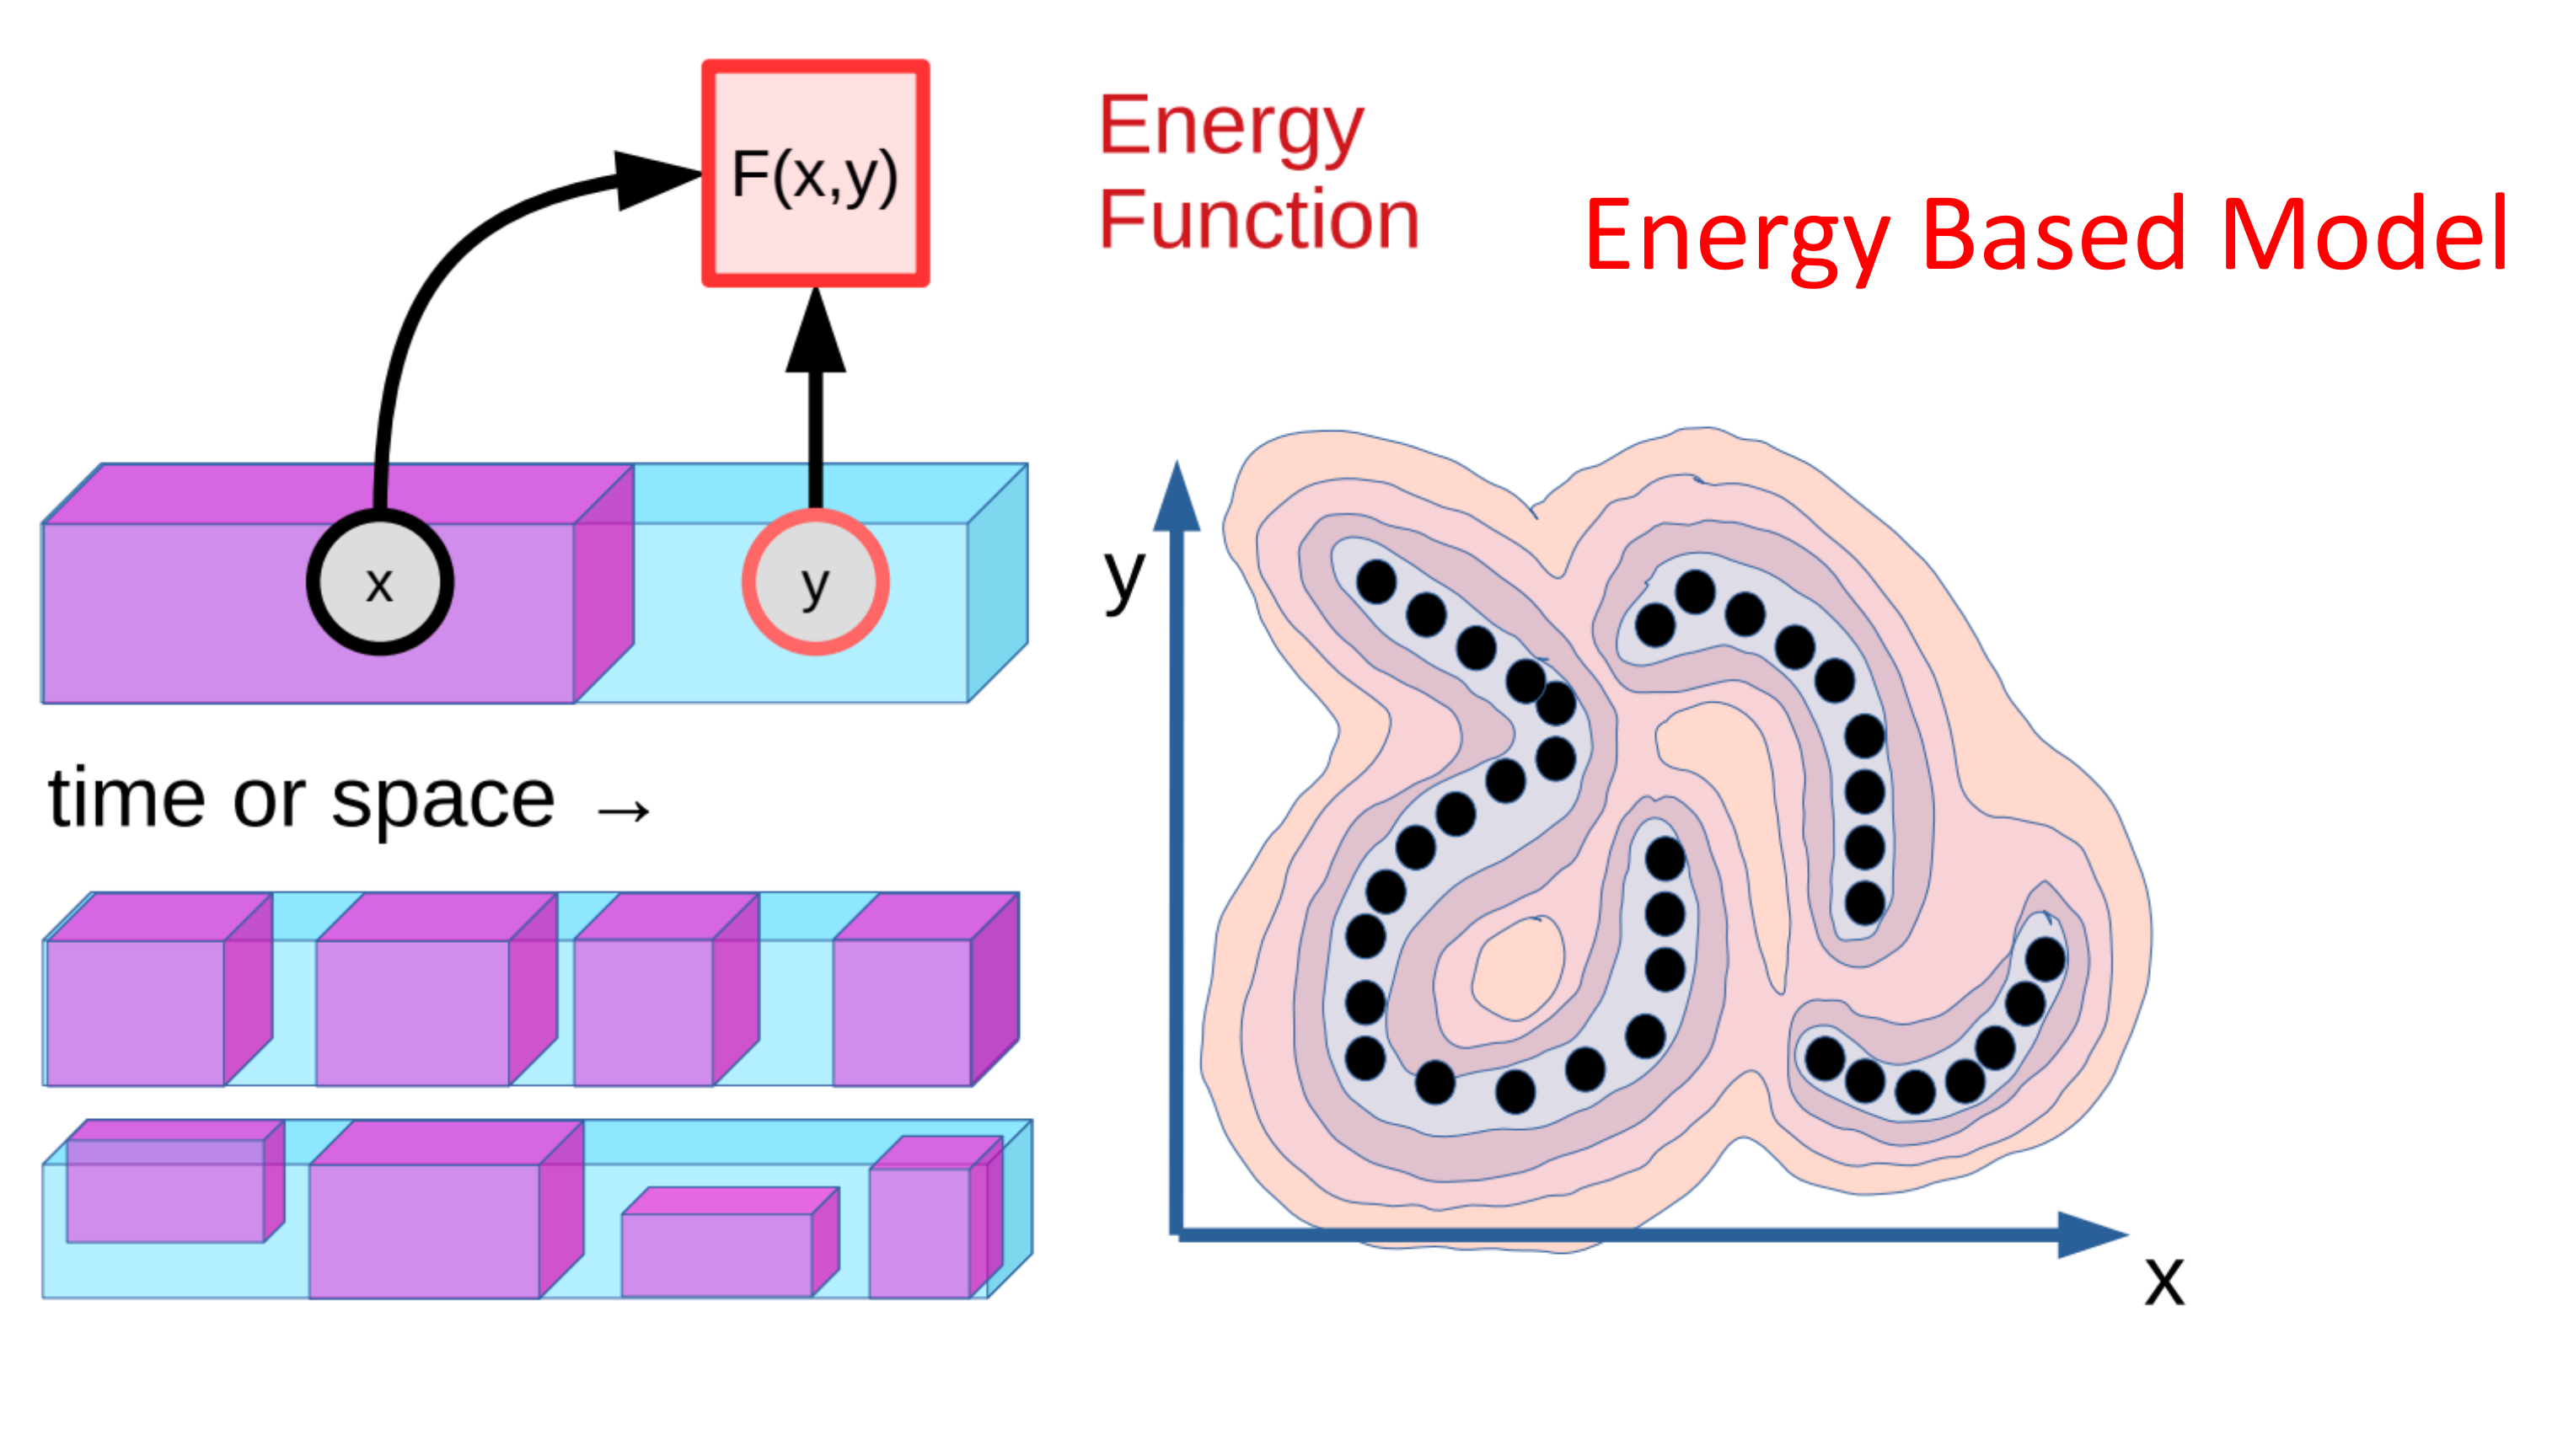
\includegraphics[width=\linewidth,height=0.82\textheight,keepaspectratio]{assets/New-Lecture_World_Models/jepa_cs25_sl06_jepa_lecun_2022_ebm.png}\\[0.08em]
  {\scriptsize Paper: \href{https://openreview.net/forum?id=BZ5a1r-kVsf}{OpenReview}, Y.\ LeCun (2022).}
\end{frame}

\begin{frame}[t]{V-JEPA: video JEPA}
  \centering
  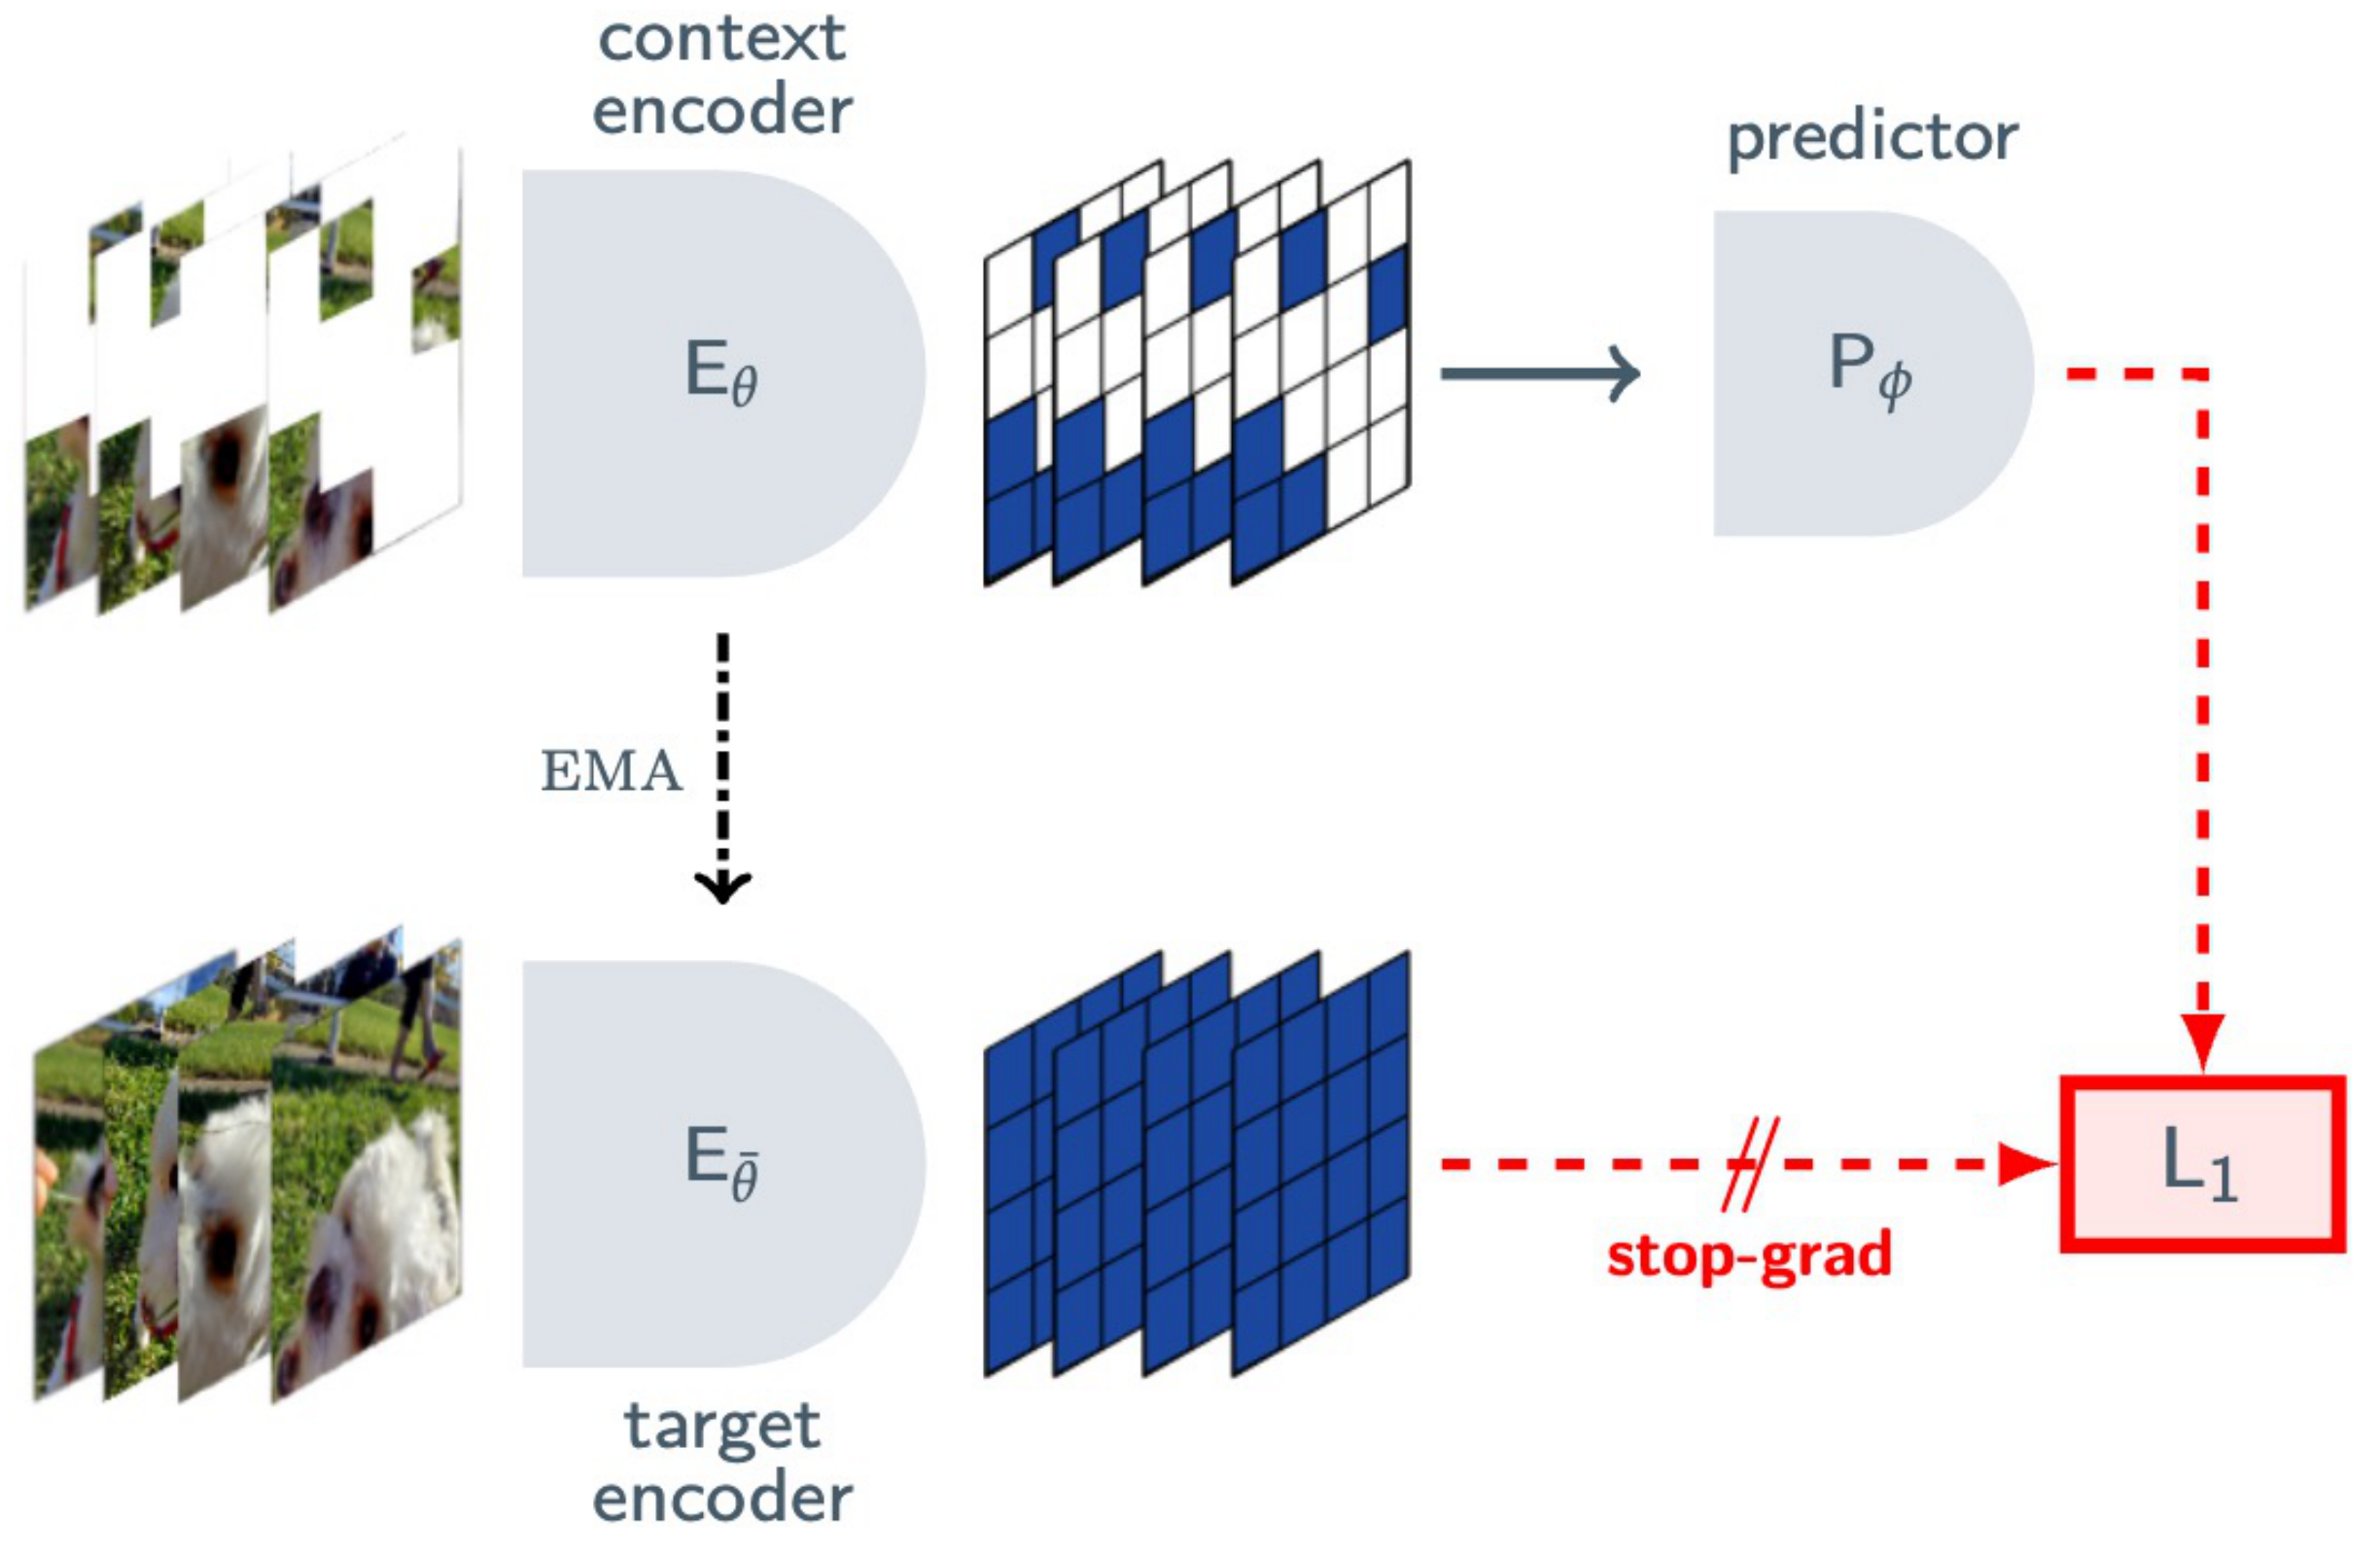
\includegraphics[width=\linewidth,height=0.82\textheight,keepaspectratio]{assets/New-Lecture_World_Models/jepa_cs25_sl07_vjepa_bardes_2024.png}\\[0.08em]
  {\scriptsize Paper: Bardes et al., \href{https://arxiv.org/abs/2404.08471}{arXiv:2404.08471} (V-JEPA).}
\end{frame}

\begin{frame}[t]{V-JEPA\,2: action-conditioned latent prediction}
  \centering
  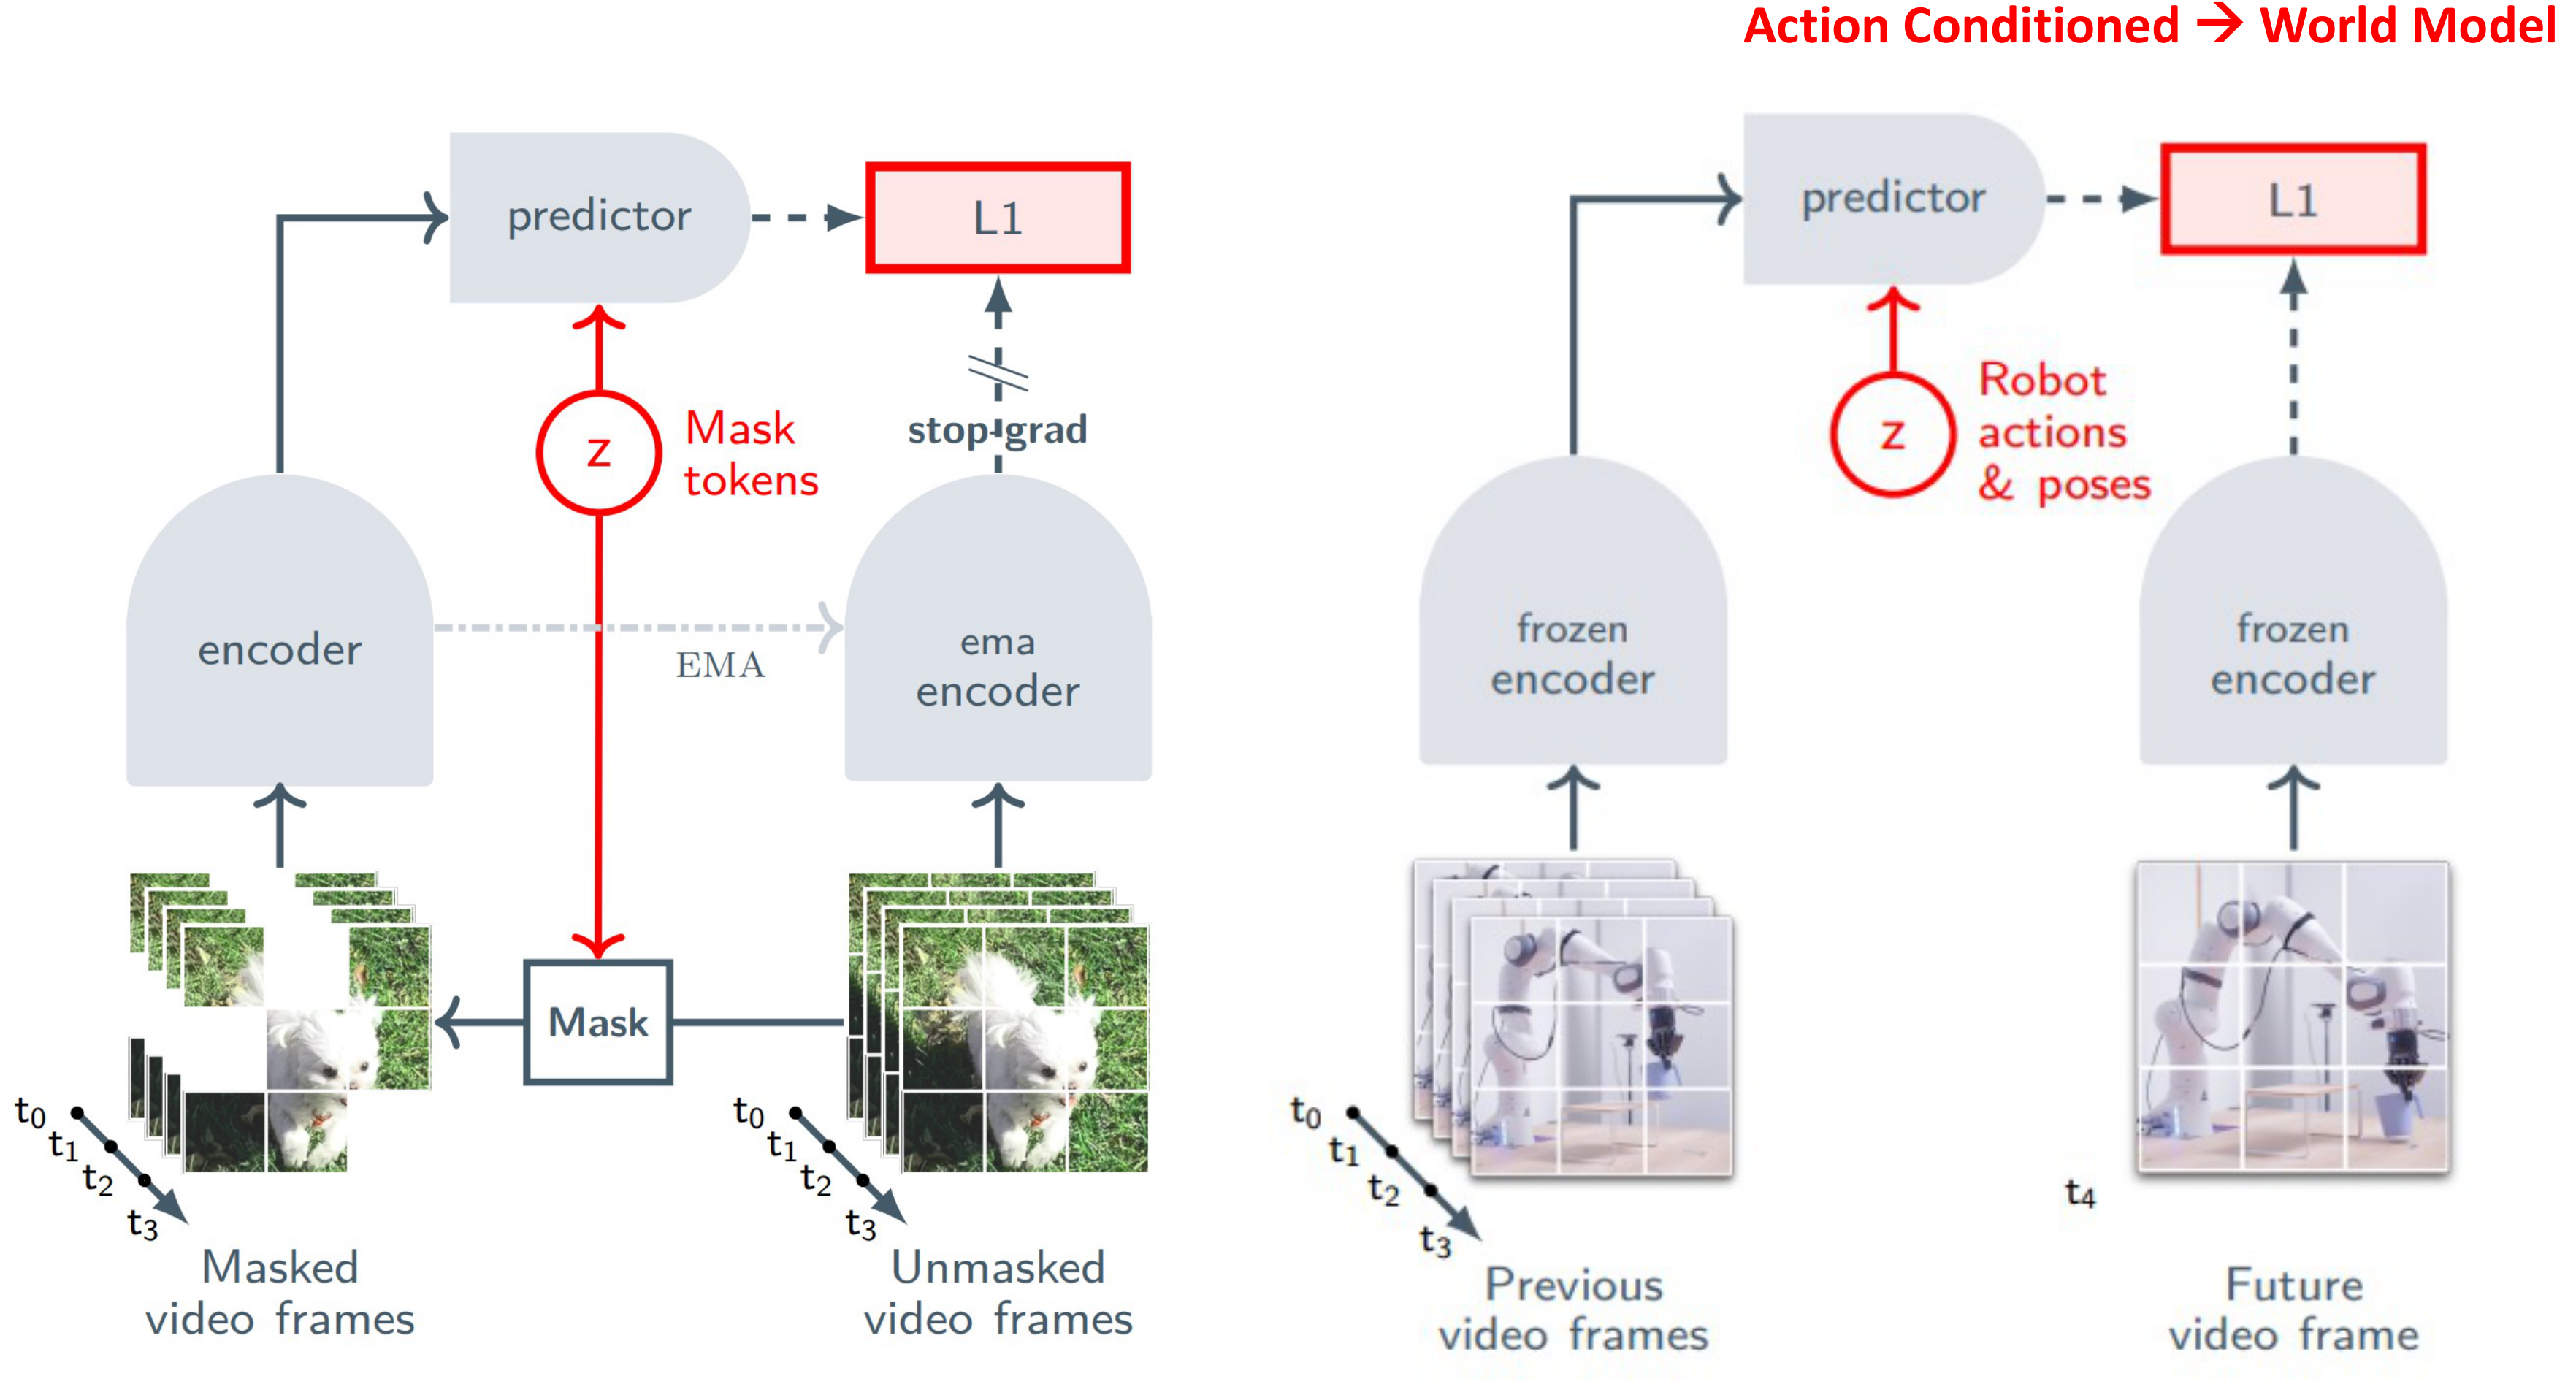
\includegraphics[width=\linewidth,height=0.74\textheight,keepaspectratio]{assets/New-Lecture_World_Models/jepa_cs25_sl08_vjepa2_action_world_model.png}\\[0.04em]
  {\scriptsize Paper: Assran et al., \href{https://arxiv.org/abs/2506.09985}{arXiv:2506.09985} (V-JEPA\,2).}
\end{frame}

\begin{frame}{Generative world models vs.\ JEPA-style prediction}
  \begin{columns}[T,onlytextwidth]
    \column{0.48\textwidth}
    \textbf{Generative (reconstruction) path}\\[0.35em]
    \begin{itemize}\itemsep0.28em
      \item[\textcolor{red}{$\blacktriangleright$}] Learn latents that \textbf{decode} back to pixels (VAE/RSSM).
      \item[\textcolor{red}{$\blacktriangleright$}] Strength: full \textbf{observation model} for planning, denoising, and imagined rollouts with explicit images.
      \item[\textcolor{red}{$\blacktriangleright$}] Cost: optimization can emphasize pixels over semantics.
    \end{itemize}
    \column{0.48\textwidth}
    \textbf{Joint-embedding predictive (JEPA) path}\\[0.35em]
    \begin{itemize}\itemsep0.28em
      \item[\textcolor{red}{$\blacktriangleright$}] Predict \textbf{embeddings} of future or masked regions in \textbf{representation space}.
      \item[\textcolor{red}{$\blacktriangleright$}] Strength: can learn useful \textbf{video/robotics} features without needing to generate every pixel.
      \item[\textcolor{red}{$\blacktriangleright$}] Cost: requires clear action input (e.g.\ V-JEPA 2-AC, LeWM).
 
    \end{itemize}
  \end{columns}
\end{frame}
